\documentclass[a4paper, 11pt]{article}
%\documentclass[a4paper, 10pt]{amsart}

% multi-line spacing for easier marking
%\usepackage{setspace}

% math symbols
\usepackage{amssymb,amsmath}
\usepackage{textcomp}

% nicer fonts
\usepackage{times}

% for fancy tables with multi-row headers
\usepackage{multirow}
% for pictures
\usepackage{graphicx}
\usepackage{wrapfig}

\usepackage{url}
\usepackage{enumitem}
\usepackage{fancyvrb}

% if appending entire pdf docs (e.g. appendix)
%\usepackage{pdfpages}

% narrow margins 
\usepackage[top=2cm, bottom=2cm, left=2cm, right=2cm]{geometry}
% no indention of paragraphs
\setlength{\parindent}{0in}
% have wider spacing between paragraphs
\setlength{\parskip}{1ex plus 0.5ex minus 0.2ex}
% greater separation between columns
\setlength{\columnsep}{0.7cm}

% handy macro defines
	% code command
\newcommand{\codeCommand}[1]{\texttt{#1}}
	% code 'type' word
\newcommand{\codeType}[1]{\textbf{\texttt{#1}}}

% for code listings, etc.
\usepackage{listings}
\usepackage{color}

\lstset{captionpos=b,tabsize=4,frame=lines,keywordstyle=\color{blue}\bf,commentstyle=\color{OliveGreen},stringstyle=\color{red},numbers=left,numberstyle=\tiny,numbersep=5pt,breaklines=true,showstringspaces=false,basicstyle=\ttfamily\footnotesize,emph={label}}

% titles stuff 
\title{\textbf{COSC427 Assignment 2} \\ {\textit{Sudoken} - User Manual}}
\author{
	Kevin Doran    \\ 33439377 \and
	Adam Freeth    \\ 68895971 \and
	Timothy Hobbs  \\ 39986601 \and
	Joshua Leung   \\ 46308424 \and
	Michael McGee  \\ 74188139
}

\begin{document}
\maketitle

%\doublespacing % for easier marking

%\section{Introduction}
% Intro
This document describes the design patterns used in a extensible solver for grid-based number puzzles such as Sudoku, Futoshiki, and Jigsaw Sudoku. A plugin architecture is used to support runtime composition and extension of the set of supported puzzle types, with plugins for additional puzzle types able to be automatically detected and loaded without (lowlevel) user intervention.

... todo: summary of key components ...

\begin{wrapfigure}{r}{0.5\textwidth}
  \begin{center}
    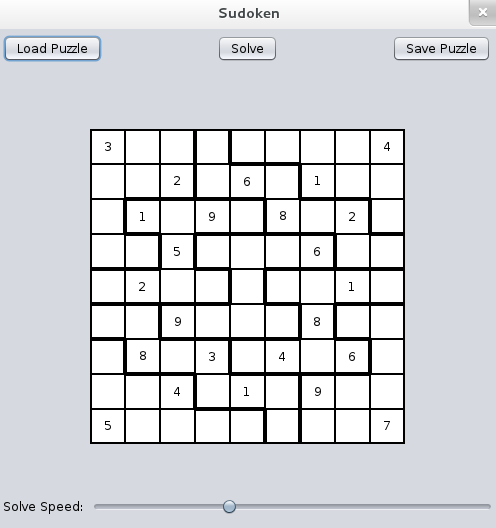
\includegraphics[width=0.48\textwidth]{gui.png}
  \end{center}
  \vspace{-10pt}
  \caption{The main Sudoken GUI.}
  \vspace{-60pt}
\end{wrapfigure}

\section{Installation}
% Installation
Unzip all files and run. % PLACEHOLDER!!!

... Prerequisites List ...

\section{Execution}
Upon running the Sudoken application, you will be presented with the GUI shown in figure TODO. Initially there will be no sudoken puzzle loaded.


\end{document}
